\documentclass[../../main.tex]{subfiles}

%-----------------------------------------------------------%
\begin{document}
\section{Configurational Layout}
\subsection{Mechanical Specifications}
\begin{enumerate}
    \item \textbf{Software:} SolidWorks 2019 is used for CAD modelling.
    \item \textbf{Model name:} STD0010002
    \item \textbf{Axes of the system:}
    \begin{table}[h!]
        \centering
        \begin{tabular}{| p{2cm} | p{7cm} |}
             \hline
             +X Axis & Arbitrarily chosen to be perpendicular to Z Axis \\
             \hline
             +Y Axis & Arbitrarily chosen to be perpendicular to Z Axis\\
             \hline
             +Z Azix & Along +ve direction of Optics system\\
             \hline
        \end{tabular}
        \caption{Axes}
        \label{tab:my_label}
    \end{table}
        \item \textbf{Components to be incorporated into STADS:}
        \begin{enumerate}
            \item \textbf{Solid Rod with Spacers Model STD0010002}
            \begin{table}[h!]
        \centering
        \begin{tabular}{| p{5cm} | p{3cm} |}
             \hline
             \textbf{Component Name} & \textbf{Quantity}  \\
             \hline
             Electrical PCB & 2 \\
             \hline
             Optics System \& PCB & 1\\
             \hline
             Side Panels & 4 \\
             \hline
             Top Panel & 1 \\
             \hline
             Bottom Panel & 1 \\
             \hline
             Solid Rods & 4 \\
             \hline
             Spacers & 16 \\
             \hline
        \end{tabular}
        \caption{Components - Solid Rod with Spacers Model}
        \label{tab:my_label}
    \end{table}
    \item \textbf{Support Rails Model STD0020001\_01}
    \begin{table}[h!]
        \centering
        \begin{tabular}{| p{5cm} | p{3cm} |}
             \hline
             \textbf{Component Name} & \textbf{Quantity}  \\
             \hline
             Electrical PCB & 2 \\
             \hline
             Optics System \& PCB & 1\\
             \hline
             Side Panels & 4 \\
             \hline
             Top Panel & 1 \\
             \hline
             Bottom Panel & 1 \\
             \hline
             Support Rails & 4 \\
             \hline
        \end{tabular}
        \caption{Components - Support Rails Model}
        \label{tab:my_label}
    \end{table}
        \end{enumerate}
    
    \begin{figure}[H]
        \centering
        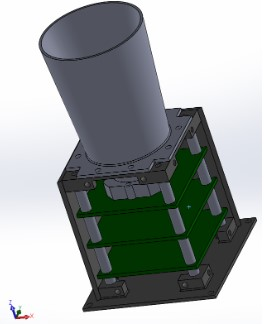
\includegraphics{Figures/Mechanical/stads_full.jpg}
        \caption{STADS CAD Model}
        \label{fig:sys_CAD}
    \end{figure}
    \begin{figure}[H]
        \centering
        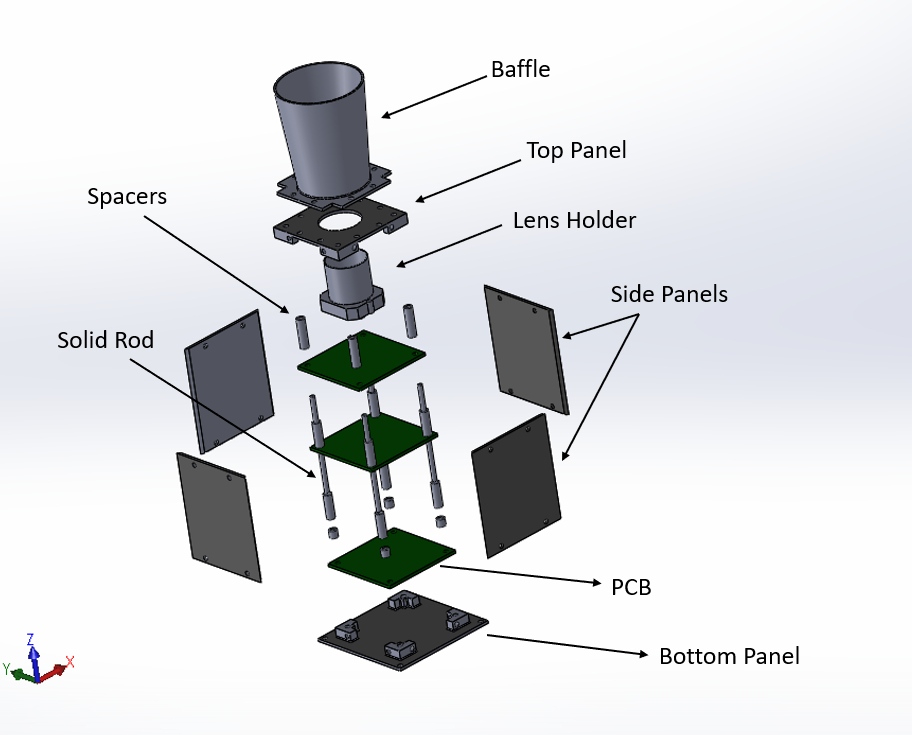
\includegraphics[scale=0.5]{Figures/Mechanical/exploded.png}
        \caption{Exploded View}
        \label{fig:sys_CAD}
    \end{figure}
    \end{enumerate}
    \subsection{Current Layout}
    \text{The STADS module is broken down into stacked components and face mounted components.}
    \begin{enumerate}
        \item \textbf{Stacked Components:} PCBs belonging to Electrical and Instrumentation subsystem are stacked inside STADS using solid rods and spacers. All components of Optics other than Baffle is connected to STADS through Optics PCB. Here 4 solid rods run through all the PCBs symmetrically. Spacers are used to keep PCBs and Panels vertically distant as required.
        \begin{figure}[H]
        \centering
        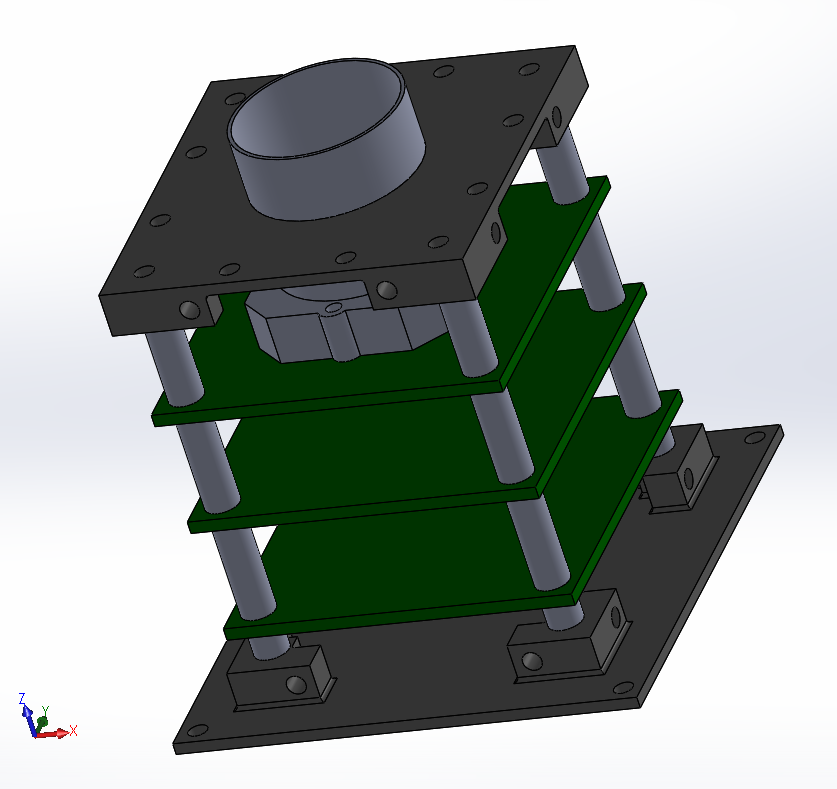
\includegraphics[scale=0.5]{Figures/Mechanical/stacked.png}
        \caption{STADS CAD Model}
        \label{fig:sys_CAD}
    \end{figure}
    \newpage
    \item \textbf{Face mounted:} Face mounted components include Panels and the Baffle.
        \begin{figure}[H]
        \centering
        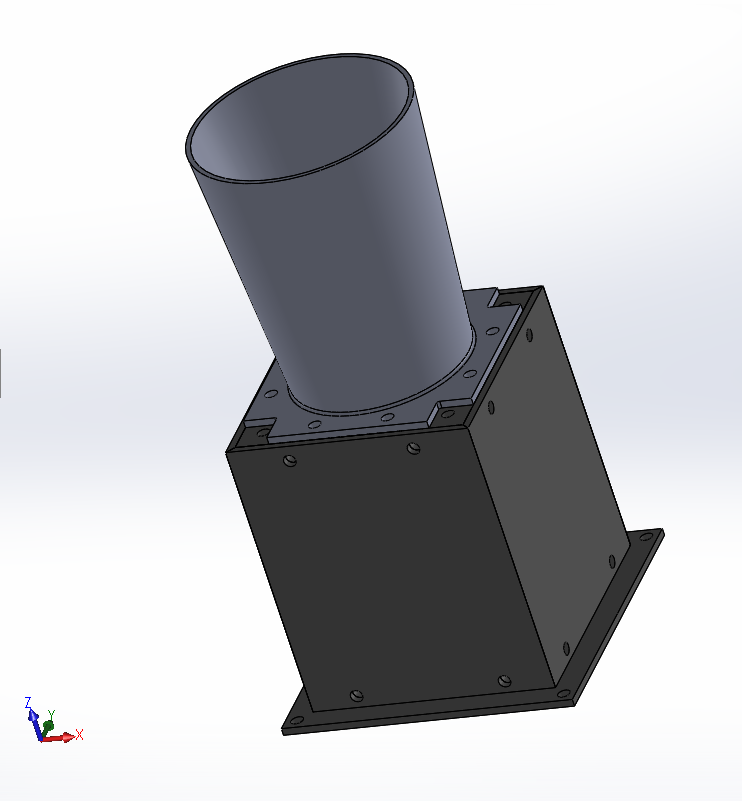
\includegraphics[scale=0.5]{Figures/Mechanical/side.png}
        \caption{Face Mounted Components}
        \label{fig:sys_CAD}
    \end{figure}
          
    \begin{enumerate}
    \item Baffle and Top Panel: Baffle is directly connected to the Top Panel using 8 screws. A centre hole on top panel also exist for sight of Optics sensor.
  
        \begin{figure}[H]
        \centering
        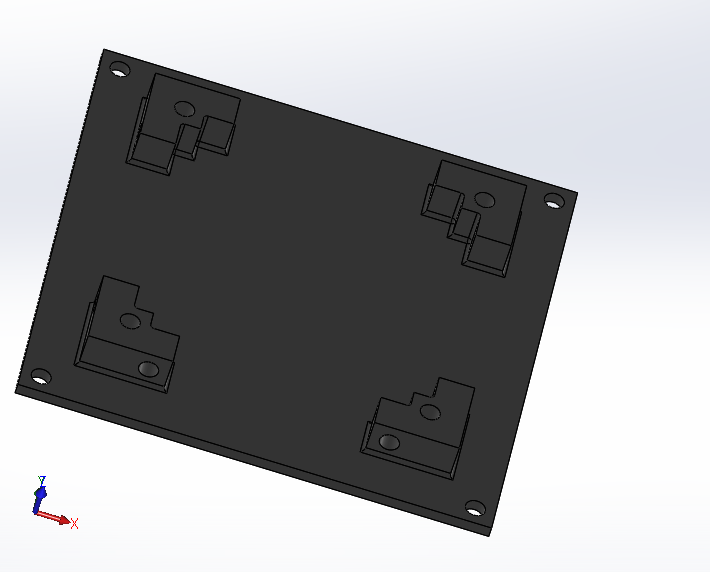
\includegraphics[scale=0.5]{Figures/Mechanical/bottom.png}
        \caption{Bottom Panel}
        \label{fig:sys_CAD}
    \end{figure}
  
    \item Bottom Panel: Acts as a mechanical interface to the user satellite and interfacing Side panels. It also act as a starting block for stacking of the PCBs.
        \begin{figure}[H]
        \centering
        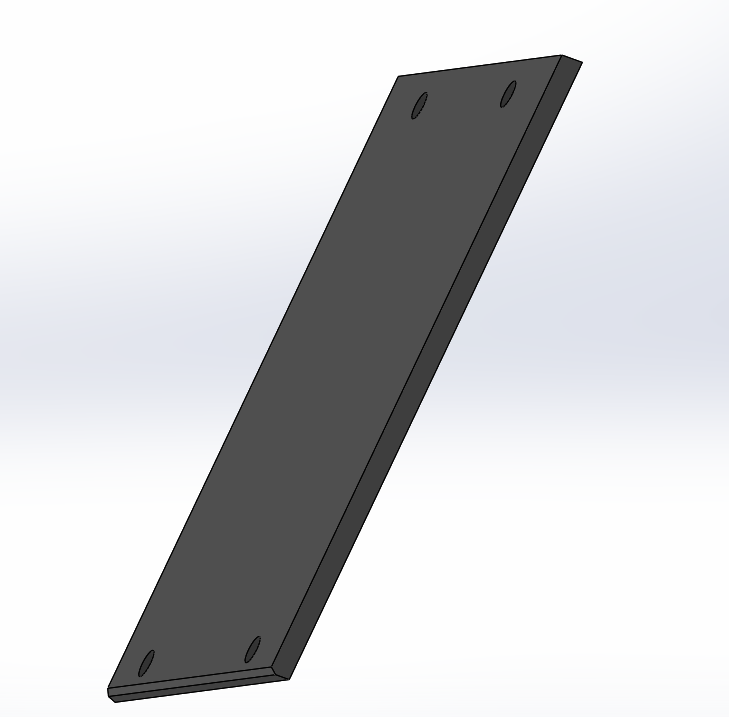
\includegraphics[scale=0.5]{Figures/Mechanical/side_panel.png}
        \caption{Side panel}
        \label{fig:sys_CAD}
    \end{figure}
    \item Side Panels: Each Side panel is interfaced with 2 screws on Top panel and Bottom Panel. These have 2 purposes of providing radiation shielding and structural stability. Further modification to incorporate connectors in our system can be done on these
    
        
      

    \end{enumerate}   
   \end{enumerate}
   \newpage
    \subsection{ \textbf{Parallel Layout:}}
    \text We have explained and shown only critical parts of the CAD, rest of the parts are similar to as shown above in the sections above.
    \begin{enumerate}
        \item \textbf{Stacking with support rail:} In this configuration stacking of PCB is done using stubs present on support rails. Also the interface of all panels is done to these support rails.
        \begin{figure}[H]
        \centering
        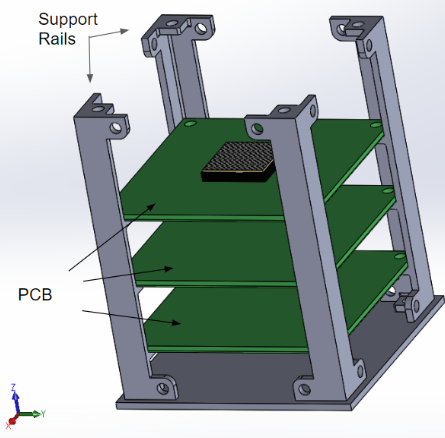
\includegraphics[scale=0.75]{Figures/Mechanical/support_stack.png}
        \caption{Support rail}
        \label{fig:sys_CAD}
    \end{figure}
        \item \textbf{Top Panel with Extruded Stubs:} In this configuration mechanical interfacing with user satellite is done using Extruded Stubs present on Top panel.
        \begin{figure}[H]
            \centering
            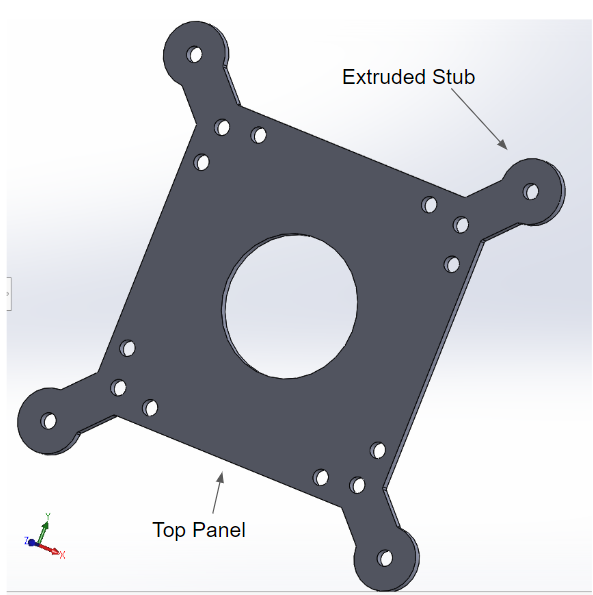
\includegraphics[scale=0.6]{Figures/Mechanical/CDR002.PNG}
            \caption{Top Panel with Extruded Stubs}
            \label{fig:sys_CAD}
        \end{figure}
        \item \textbf{Entire Assembly with Exploded Views}
        \begin{figure}[H]
            \centering
            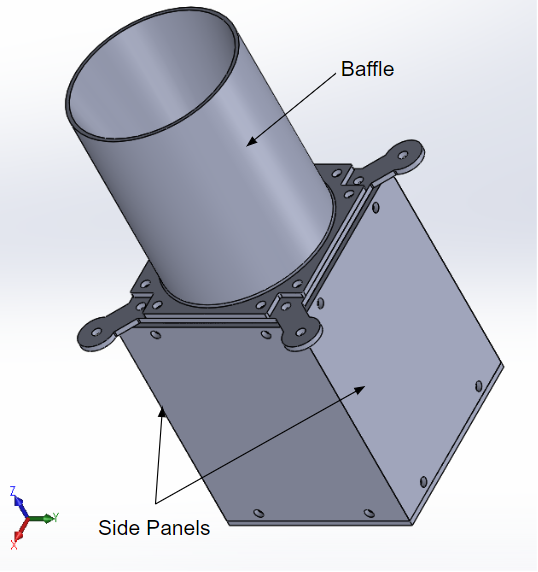
\includegraphics[scale=0.7]{Figures/Mechanical/CDR003.PNG}
            \caption{Entire Assembly}
            \label{fig:sys_CAD}
        \end{figure}
        \begin{figure}[H]
            \centering
            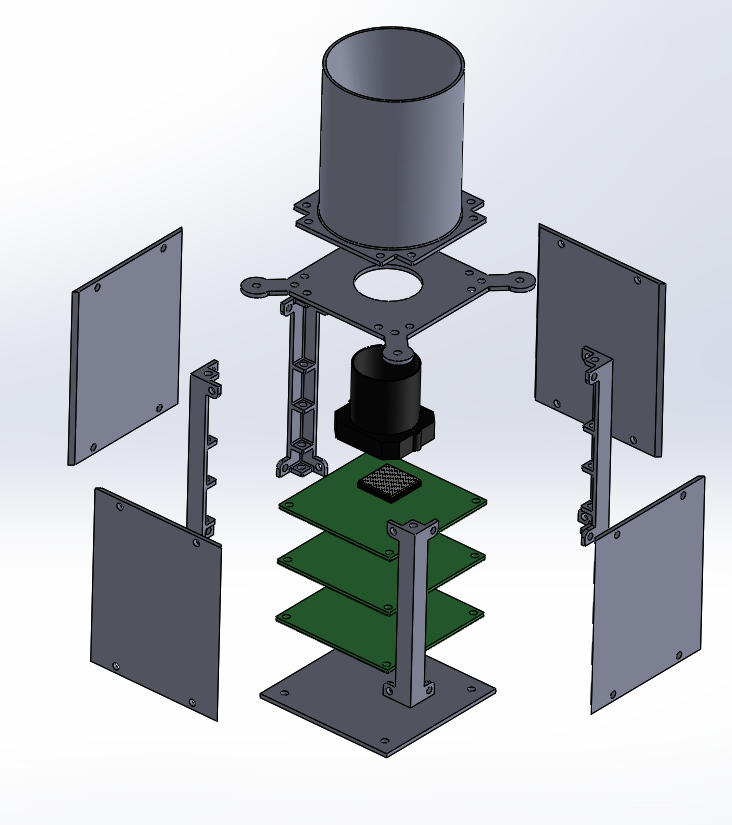
\includegraphics[scale=0.6]{Figures/Mechanical/STADS_Support_Integration.PNG}
            \caption{Exploded View of Entire Assembly}
            \label{fig:sys_CAD}
        \end{figure}
    \end{enumerate}

%----------------------------END----------------------------%
\end{document}